% Options for packages loaded elsewhere
\PassOptionsToPackage{unicode}{hyperref}
\PassOptionsToPackage{hyphens}{url}
%
\documentclass[
  11pt,
]{article}
\usepackage{amsmath,amssymb}
\usepackage{iftex}
\ifPDFTeX
  \usepackage[T1]{fontenc}
  \usepackage[utf8]{inputenc}
  \usepackage{textcomp} % provide euro and other symbols
\else % if luatex or xetex
  \usepackage{unicode-math} % this also loads fontspec
  \defaultfontfeatures{Scale=MatchLowercase}
  \defaultfontfeatures[\rmfamily]{Ligatures=TeX,Scale=1}
\fi
\usepackage{lmodern}
\ifPDFTeX\else
  % xetex/luatex font selection
\fi
% Use upquote if available, for straight quotes in verbatim environments
\IfFileExists{upquote.sty}{\usepackage{upquote}}{}
\IfFileExists{microtype.sty}{% use microtype if available
  \usepackage[]{microtype}
  \UseMicrotypeSet[protrusion]{basicmath} % disable protrusion for tt fonts
}{}
\makeatletter
\@ifundefined{KOMAClassName}{% if non-KOMA class
  \IfFileExists{parskip.sty}{%
    \usepackage{parskip}
  }{% else
    \setlength{\parindent}{0pt}
    \setlength{\parskip}{6pt plus 2pt minus 1pt}}
}{% if KOMA class
  \KOMAoptions{parskip=half}}
\makeatother
\usepackage{xcolor}
\usepackage[margin=1in]{geometry}
\usepackage{graphicx}
\makeatletter
\def\maxwidth{\ifdim\Gin@nat@width>\linewidth\linewidth\else\Gin@nat@width\fi}
\def\maxheight{\ifdim\Gin@nat@height>\textheight\textheight\else\Gin@nat@height\fi}
\makeatother
% Scale images if necessary, so that they will not overflow the page
% margins by default, and it is still possible to overwrite the defaults
% using explicit options in \includegraphics[width, height, ...]{}
\setkeys{Gin}{width=\maxwidth,height=\maxheight,keepaspectratio}
% Set default figure placement to htbp
\makeatletter
\def\fps@figure{htbp}
\makeatother
\setlength{\emergencystretch}{3em} % prevent overfull lines
\providecommand{\tightlist}{%
  \setlength{\itemsep}{0pt}\setlength{\parskip}{0pt}}
\setcounter{secnumdepth}{5}
\usepackage{booktabs}
\usepackage{longtable}
\usepackage{array}
\usepackage{multirow}
\usepackage{wrapfig}
\usepackage{float}
\usepackage{colortbl}
\usepackage{pdflscape}
\usepackage{tabu}
\usepackage{threeparttable}
\usepackage{threeparttablex}
\usepackage[normalem]{ulem}
\usepackage{makecell}
\usepackage{xcolor}
\ifLuaTeX
  \usepackage{selnolig}  % disable illegal ligatures
\fi
\usepackage{bookmark}
\IfFileExists{xurl.sty}{\usepackage{xurl}}{} % add URL line breaks if available
\urlstyle{same}
\hypersetup{
  pdftitle={Vance County EMS Station Analysis Report},
  pdfauthor={Alayna Binder, Cindy Ju, Kathleen Zhang},
  hidelinks,
  pdfcreator={LaTeX via pandoc}}

\title{Vance County EMS Station Analysis Report}
\author{Alayna Binder, Cindy Ju, Kathleen Zhang}
\date{2025-10-21}

\begin{document}
\maketitle

{
\setcounter{tocdepth}{2}
\tableofcontents
}
\section{Background}\label{background}

Without an effective distribution of emergency medical resources,
counties risk delayed response times that can mean the difference
between life and death. To improve coverage across Vance County,
researchers analyzed data from the county's EMS system, which currently
operates four ambulances from two stations located in the Central and
South districts. Historical records show that residents in the North
district face much longer response times, often averaging over 12
minutes, compared to 6 and 9 minutes in the Central and South regions.

Using a dataset of recorded EMS trips containing call locations,
dispatch and arrival times, and Google API travel estimates, this
analysis evaluates how different station configurations and vehicle
allocations affect system performance. The county is considering
establishing a new station in the North district, with two potential
site options (Near North and Far North), and several ambulance
distribution scenarios.

Our goal is to determine which North station location would most
effectively reduce response times and how the four available ambulances
should be allocated among the stations to balance coverage and minimize
system strain. We aim to illustrate this through visual and numerical
summaries that highlight tradeoffs in travel time and resource
availability across the scenarios.

\section{Data and Exploratory
Analysis}\label{data-and-exploratory-analysis}

\subsection{Data}\label{data}

We were given 489 observations of calls occurring in Vance County
between January 1st to January 25th in 2024.

One of the calls went to Duke Hospital, which we excluded. Additionally,
in certain incidents where multiple patients were involved, they would
be transported in the same ambulance. As we only care about the
availability of ambulances and not how many patients were in a single
ambulance, we cleaned the dataset so that every identical row
represented a single, unique incident involving one ambulance. The
identical condition ensured datapoints where multiple ambulances were
sent out for one incident with multiple patients would still be in the
dataset, as it would impact ambulance load.

\subsection{Exploratory Data Analysis}\label{exploratory-data-analysis}

To understand where and when ambulance demand occurs, our EDA began with
plotting a call-density map (Figure 1) that showed a clear cluster
around the Central station with spread in the South and scatter in the
North, motivating scenarios that add northern coverage. We then compared
Near North vs.~Far North (Figure 2) calls, and found that using Google's
UA travel times, Near North was closer for 90\% of northern calls, cut
response time by about 4 minutes on average relative to Far North, and
had shorter total call duration with quicker transportation to
hospitals.

\section{Modeling}\label{modeling}

\subsection{Simulating the Data}\label{simulating-the-data}

The objectives are to compare different scenarios to determine the
optimal options for station placement as well as ambulance allocations,
but we do not have data about ambulance response times under different
station locations and ambulance allocations. As a result, we conducted a
simulation that would simulate response times for each of the five
scenarios for every single call in our cleaned dataset, resulting in 5
observations for every original call.

We developed Scenario Dispatch Rules that would govern how the
simulation responded to different scenarios.

From our exploratory data analysis, we determined that we wanted to
consider scenarios where an ambulance might not be available. Therefore,
in our rules, each incoming call first checks whether any ambulances are
currently available. If at least one unit is free, the system assigns
the closest available unit --- the one with the smallest estimated
travel time, based on Google's best-guess ETA between that station and
the call location, resulting in 0 wait time. If all units are busy, the
call enters a queue and waits until the next ambulance becomes free.
That waiting time is then added to the total response time. Once
assigned, each unit stays occupied for the observed duration of the
call, and then becomes available again for the next incident.

The wait time is determined by whether or not an ambulance unit is
available at the moment an incident call comes in. This models the
effect of queueing for service. The wait time is calculated based on two
conditions:

If one or more units are already free when the call arrives, we assign
the closest available unit, which is the one with minimum ETA. The unit
is dispatched immediately at the call time, resulting in zero wait time.

Otherwise, if all units are busy when the call arrives, we assign the
unit that is scheduled to become free soonest. The wait time is the time
difference between the call time and the departure time, which is the
time the assigned unit finally becomes free. This represents the
queueing delay. In both cases, the unit's subsequent availability is
updated by adding the observed service duration to its departure time,
making the unit busy for the duration of the incident.

Finally, we calculate Total Response Time or simulated time as Wait Time
+ Travel Time.

We filtered the results to exclude extremely long simulated times (above
2000 seconds) to focus on more likely outcomes. We also added a
variable, ``switched'', which determines if the ambulance assigned in a
new scenario (S1−S4) is different from the baseline assignment (S0).

\subsection{Model Selection and
Rationale}\label{model-selection-and-rationale}

We chose to use a linear mixed model with a fixed effect on Scenario,
which allowed us to calculate and test the difference in the mean
simulated response time between our five Scenarios (S0 through S4), as
one of the primary objectives was determining changes in response time
across different scenarios.

We also included a random intercept for Incident\_ID, allowing every
unique incident to have its own baseline average response time that
differs from the overall mean, even before accounting for the Scenario.

We fit a preliminary model with just these two components, but it had a
lot of heteroscedasticity in the residuals plot. Therefore, we added a
variance function that allows the remaining unexplained variability in
response time to be different for each Scenario. If a scenario has a
high residual variance, it means that even after controlling for the
mean, its response times are highly unpredictable or erratic. Meanwhile,
if a scenario has a low residual variance, it indicates highly
consistent service performance, which is generally desirable in a
real-world context.

Thus, our final model was:

\[\text{sim\_time}_{ij} = \beta_0 + \sum_{k=1}^4 \beta_k \cdot I(\text{Scenario}_j = S_k) + u_i + \epsilon_{ij} \]

\[
u_i \sim N(0, \sigma^2_u)\text{, }\epsilon_{ij} \sim N(0, \sigma^2)
\]

where \(\sigma^2_j = \sigma^2 \cdot\delta^2_j\)

\(\text{sim_time}_{ij}\) is the simulated response time for the \(i\)-th
Incident ID under the \(j\)-th Scenario.

\(u_i\) is the random intercept for the \(i\)-th Incident ID.
\(\sigma^2_j\) is the residual variance specific to the \(j\)-th
Scenario, which is impacted by our variance parameter \(\delta_j^2\)
that scales the baseline variance for Scenario \(j\).

\subsection{Model Implementation}\label{model-implementation}

Linear mixed models were fit in R using the \texttt{nlme} package.
Additionally, we ended up dropping data where simulated time was the
same across all scenarios in order to focus on the effect of changes
resulting from the different Scenarios.

\subsection{Model Evaluation}\label{model-evaluation}

Dropping the data where simulated time was the same across all scenarios
resulted in a lower AIC and BIC of the model fitted on the reduced
dataset compared to the non-reduced dataset.

We also examined a QQ plot which appears approximately normal. Our
Normalized Residuals vs Fitted Values plot of the total response time
appears randomly distributed.

We also looked at the Residuals vs Fitted by Scenario, where the points
in red indicate calls where the assigned station under the simulation
was different from the assigned station in our original dataset.

\section{Model Results}\label{model-results}

The intercept term is the estimated mean simulated total response time
for the reference group, Scenario 0, which is the current distribution
of ambulances and stations. The mean response time in S0 is
approximately 470.22 seconds or 7 minutes, 50 seconds. This value is
highly significant, with a p-value \textless{} 0.001 .

The mean simulated total response time in Scenario 3 is estimated to be
60.96 seconds faster than in Scenario 0, with this being a significant
difference.

\section{Conclusion, Shortcomings and Future
Work}\label{conclusion-shortcomings-and-future-work}

\subsection{Conclusion}\label{conclusion}

After evaluating five ambulance deployment layouts across the county by
replaying the same 489 incidents under each scenario with a dispatch
rule (sending the closest available unit, if none are free, dispact the
next free unit when it is available), our analysis showed that Scenario
3, which locates one ambulance in the Near North, two ambulances in the
Central, and one ambulance in the South, perfomed best. Across mean and
median response times, Scenario 3 reduced average response time the most
and produced the highest share of calls meeting eight and ten minute
targets. These results are consistent with intuition, where a more
balanced coverage of the county opposed to a centralized fleet lowers
typical responses and extreme delays.

\subsection{Limitations and Future
Work}\label{limitations-and-future-work}

However, one limitation to our analysis is the travel-time realism- we
used Google's unadjusted ETAs and treated them as fixed, so rush hour,
weather, and road disruptions are not modeled, which underestimates our
variability. Additionally, there was no priority handling and all calls
were treated the same, so our model is limited in analyzing how our
layouts affect critical cases vs.~low-priority calls. In the future,
additional work would involve adding time-of-day factors to travel by
multiplying ETAs by peak/off-peak multipliers, and running two queues
for emergency and non-emergency, allowing emergencies to jump ahead of
any waiting non-emergency calls when waiting for the next dispatch.

\section{Appendix}\label{appendix}

\subsection{Tables and Figures}\label{tables-and-figures}

\textbf{Figure One: Density of Calls in Vance County}

\begin{figure}
\centering
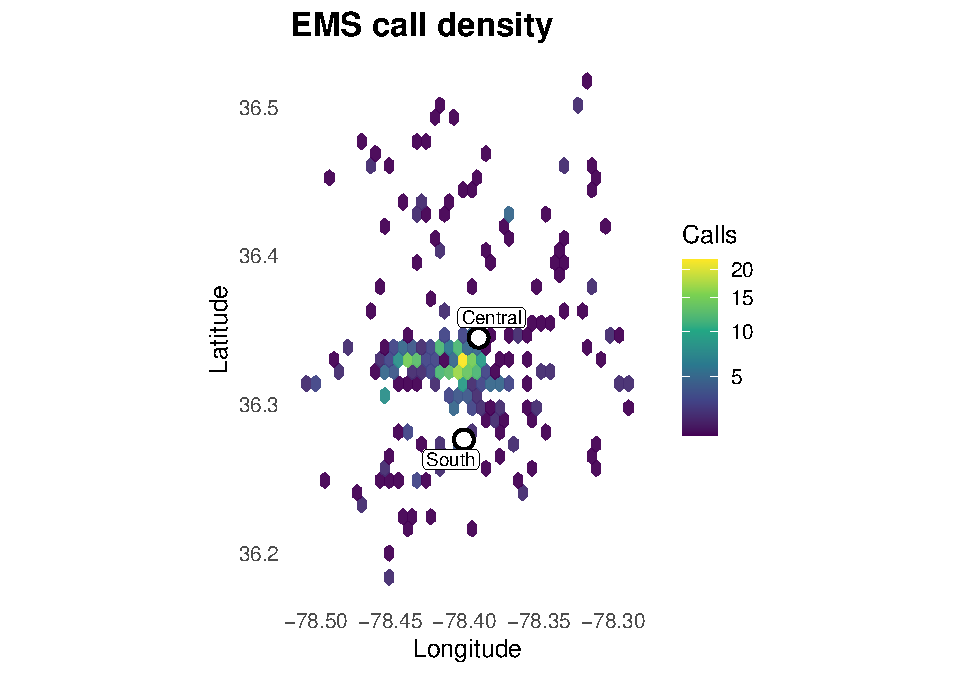
\includegraphics{Report_files/figure-latex/eda1-1.pdf}
\caption{EMS call density across Vance County (geographically)}
\end{figure}

\newpage

\textbf{Figure Two: Comparison of Near vs.~Far North Demand}

\begin{figure}
\centering
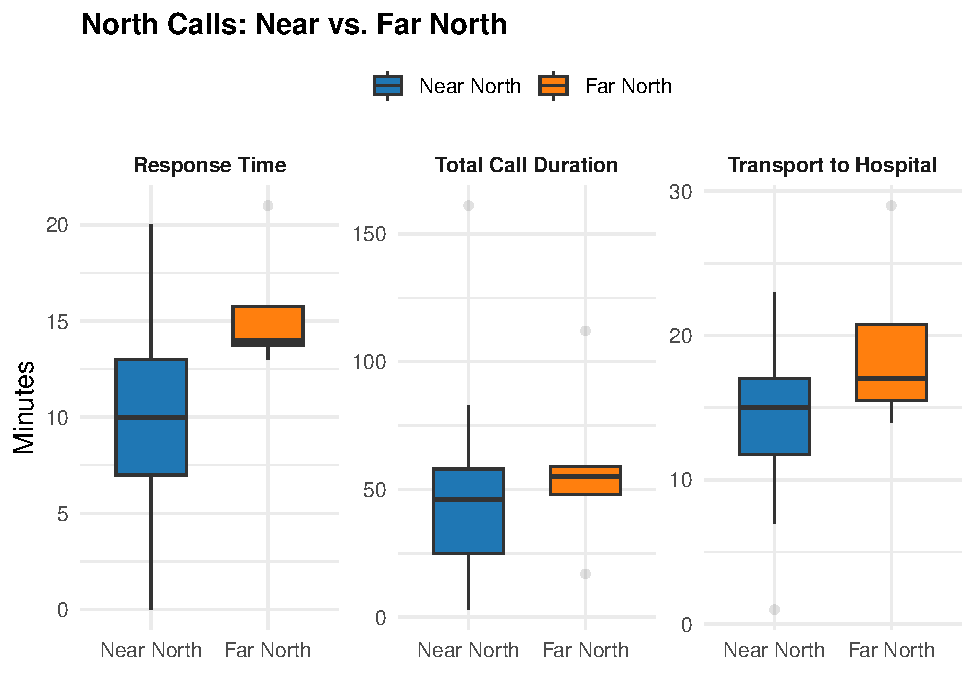
\includegraphics{Report_files/figure-latex/eda2_2-1.pdf}
\caption{test}
\end{figure}

\textbf{Figure Three: Percentage of Ambulance Utilization}

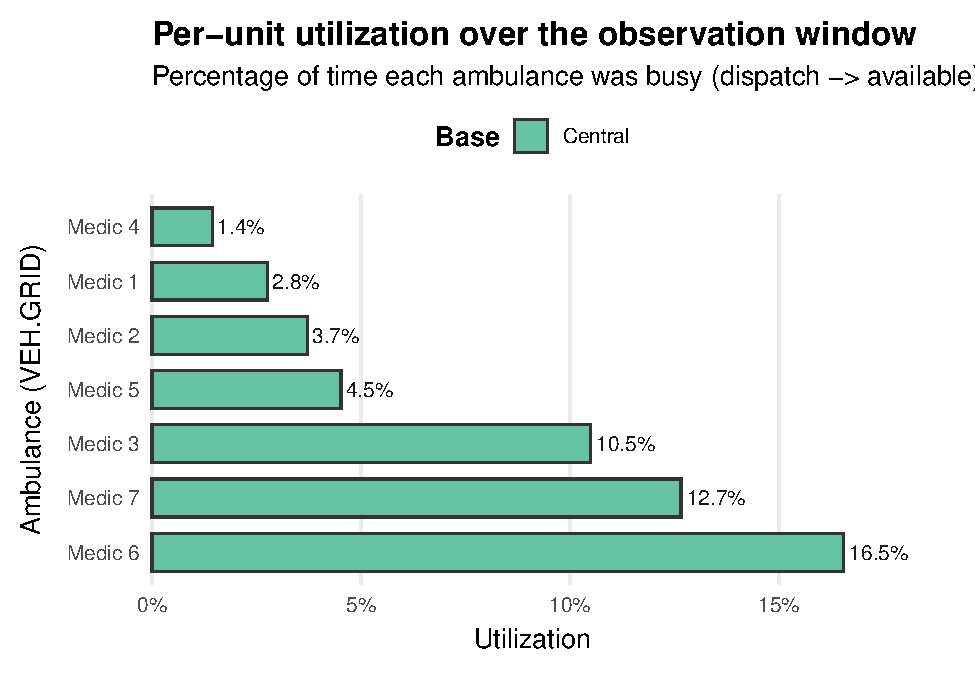
\includegraphics{Report_files/figure-latex/eda3-1.pdf}

\textbf{Figure Four: Examining Overburdening Issue}

\begin{verbatim}
## 
## Summary by region for 2024-01-16 :
## # A tibble: 3 x 6
##   region  n_calls avg_duration_min med_duration_min min_duration_min
##   <fct>     <int>            <dbl>            <dbl>            <dbl>
## 1 South         3             35.7               37                8
## 2 Central      15             27.7               20                1
## 3 North         2             60                 60               56
## # i 1 more variable: max_duration_min <dbl>
\end{verbatim}

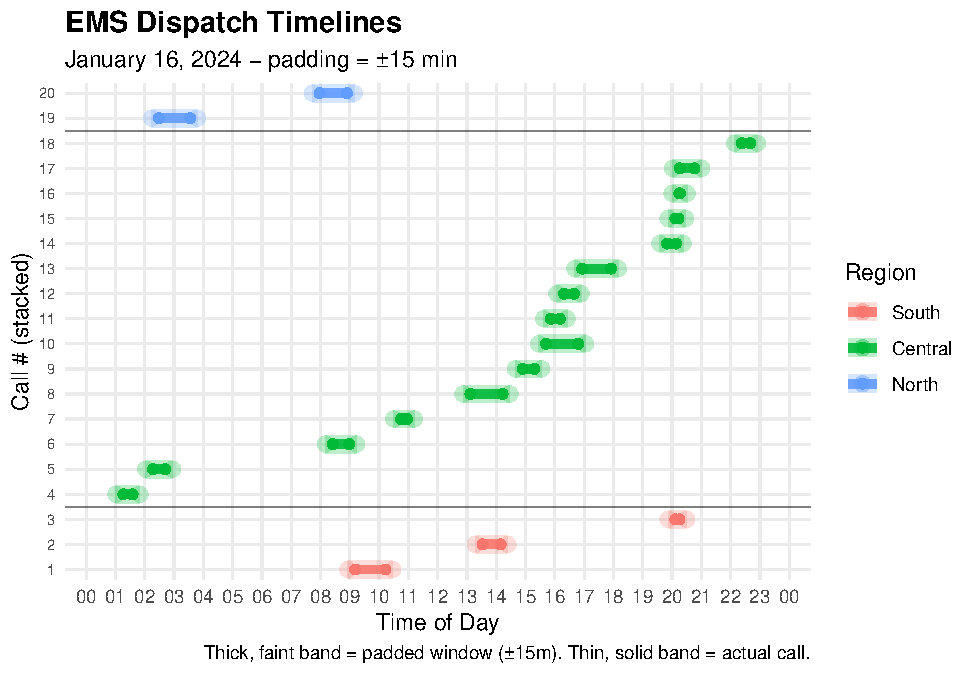
\includegraphics{Report_files/figure-latex/eda4-1.pdf}

\textbf{Figure Five: Overburdening by Region}

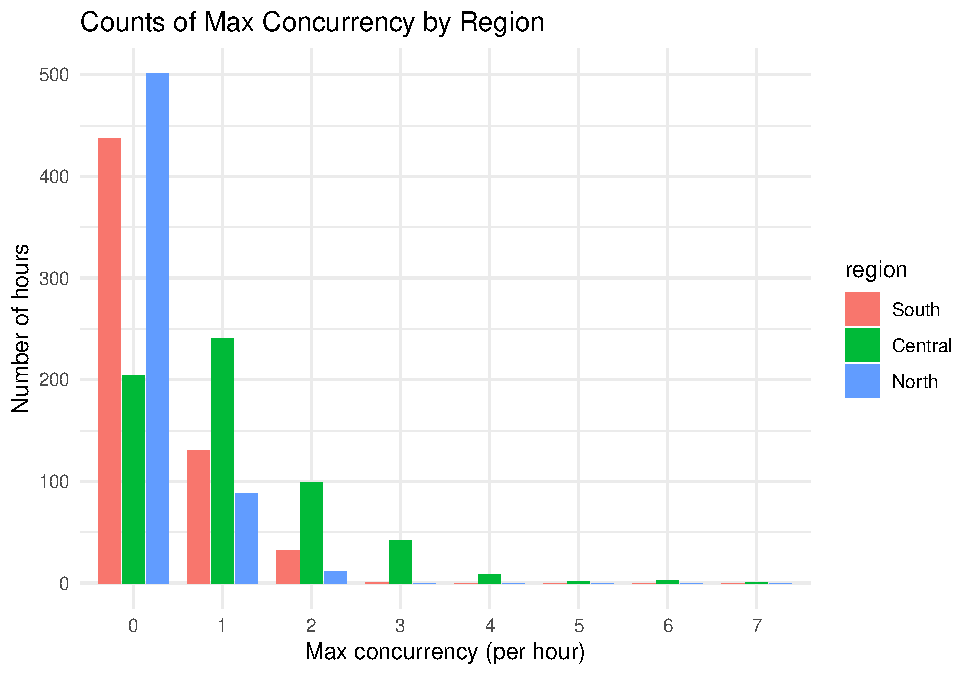
\includegraphics{Report_files/figure-latex/eda5-1.pdf}

\end{document}
